% 2009 年上海卷理科第 18 题：过圆 C 圆心的直线交 x、y 正半轴于 A、B，圆把三角形分成四部分。
% 来源 PDF：普通高考/2009/2009上海理.pdf，SHA256 82ede013bf354097cfc65c1bab2885db813572321b6eb0012f445c1c754d3fa8
% 原页：第 1 页（A3 三栏）第 2 栏下部，印刷页 553，图在题干下方。
% 重绘依据：x、y 轴正方向，圆心 C(1,1)、半径 1（与两轴相切）；直线过 C 交 x 轴于 A、y 轴于 B，
%   取 A 在右、B 在上；四个区域标 I（近 A）、II（近 O）、III（近 B）、IV（圆内 C 附近）。
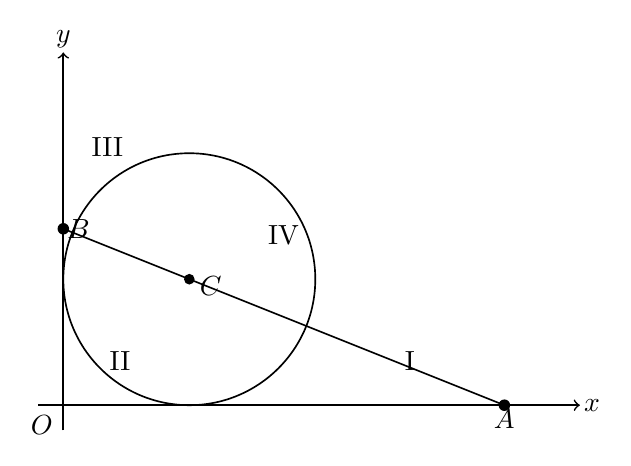
\begin{tikzpicture}[scale=1.6, semithick, every node/.style={inner sep=1.2pt}]
  \draw[->] (-0.2,0) -- (4.1,0) node[anchor=west] {$x$};
  \draw[->] (0,-0.2) -- (0,2.8) node[anchor=south] {$y$};
  \node[anchor=north east] at (-0.05,-0.05) {$O$};
  \draw (1,1) circle (1);
  \fill (1,1) circle (1.2pt);
  \node[anchor=north west] at (1.05,1.05) {$C$};
  \coordinate (A) at (3.5,0);
  \coordinate (B) at (0,1.4);
  \draw (A) -- (B);
  \fill (A) circle (1.3pt) node[anchor=north] {$A$};
  \fill (B) circle (1.3pt) node[anchor=west] {$B$};
  \node at (2.75,0.35) {$\mathrm I$};
  \node at (0.45,0.35) {$\mathrm{II}$};
  \node at (0.35,2.05) {$\mathrm{III}$};
  \node at (1.75,1.35) {$\mathrm{IV}$};
\end{tikzpicture}
